\chapter[Making the most of imperfect farm household data: a critical evaluation of standard information collected in farm household surveys]{Making the most of imperfect farm household data: a critical evaluation of standard information collected in farm household surveys}
\chaptermark{Making the most of imperfect data}
\label{cha:chapter3}
\vspace*{\fill}
Author copy of:
\\
\\
% Full citation of the published (or submitted/in review) article
% This refers to the article key in the refs.bib file.
%\bibentry{Fraval2018}
Fraval, S., Hammond, J., Wichern, J., Oosting, S. J., de Boer, I. J. M., Teufel, N., Lannerstad, M., Waha, K., Pagella, T., Rosenstock, T. S., Giller, K. E., Herrero, M., Harris, D., van Wijk, M. T. (2018). Making the most of imperfect data: a critical evaluation of standard information collected in farm household surveys. \textit{Experimental Agriculture}, 1–21. doi:10.1017/S0014479718000388.
\\
\\
Supplementary information is publically available online, accessable via the \href{https://doi.org/10.1017/S0014479718000388}{doi}.


\newpage

\section*{Abstract}
Household surveys are one of the most commonly used tools for generating insight into rural communities. These methods are frequently used in the design and evaluation of agricultural development programmes. Despite their prevalence, few studies have evaluated the quality of such data. We reviewed data from three different farm household surveys deployed in four African countries. We found issues concerning the quality of many reported values and indicators. Surprisingly, even variables which might be considered `easy to estimate' had instances of non-credible observations. Assessment of food security and food self-sufficiency showed that between 29-57\% of observations in the World Bank's 'living standards measurement survey' were deemed beyond credible bounds, while for shorter and more targeted survey tools like the `rural household multiple indicator survey' this value decreased to 25\%. Measurements of maize yields and land owned were found to be less reliable than other stationary variables. This lack of reliability has implications for monitoring food security status, poverty status and the land productivity of households. Despite this rather bleak picture, our analysis shows that if the same farm households are followed over time, the sample sizes needed to detect substantial changes are in the order of hundreds of surveys, and not in the thousands. Our research highlights the value of targeted and systematised household surveys for detecting such changes. Furthermore, ongoing developments in data collection strategies and tools are likely to improve data quality. Aspects that need sustained or improved attention include: survey design (questions and length), transparency of experimental design, effective training, improved coordination between agencies, incorporating mixed modes of data collection and ongoing systematic validation programs. Improvements in the quality of rural statistics will maximise the impact of evidence-based decision making.

\newpage

\section{Introduction}

Smallholder agricultural production in sub-Saharan Africa (SSA) remains a vital source of sustenance, revenue and employment. In the context of forecasted population growth and rapid economic development in many African nations, rural communities will have new opportunities and heightened challenges. Effective, inclusive, and poverty-reducing rural transformation is not an inevitable outcome in future scenarios for SSA nor the broader global rural population (\citealp{IFAD2016}). Rather, pro-poor and equitable rural transformation requires well designed and executed policies and interventions guided by the rural communities themselves.

Household surveys are one of the most commonly used tools for generating insights into rural communities (\citealp{Christiaensen2017}). These tools are used in place of more detailed studies because they are relatively cost-effective. The surveys rely heavily on farmer assessment and recall in place of (more detailed) external monitoring and measurement. The utilisation of low-cost farmer recall enables them to be deployed quickly and at scale which is vital for obtaining representative samples of rural communities and regions. Household surveys can be used for ex-ante and ex-post analyses. Ex-ante applications can be focused on strategic planning purposes, involving prioritisation, characterisation and simulations. Ex-post assessments measure the effect of some 'change'; typical examples include evaluation of new technologies and practices (e.g. those related to cropping, livestock production, land management and natural resource management), or changes to policies and infrastructure (e.g. new roads and market interventions). Ex-post assessments will often assess effects on productivity, decisions (farm management, investments, marketing and off-farm activities) and livelihoods (income, wealth and equity).

Evidence generated to develop and evaluate policies and interventions should be representative of the population of interest, as well as of sufficient quality. Such evidence needs to be founded on a statistically robust sampling protocol that is of sufficient size and designed to minimise sampling error (biases in respondent selection contrary to the population composition) and coverage error (biases from an incomplete sampling frame). The total measurement error of household survey data also consists of random and systematic error, caused by the implementation process of a household survey. Random error can be thought of as instances where repeated measures result in randomly inconsistent values, and systematic errors are errors that are not caused by chance but rather are consistently over or under-reported in a given measurement and observation context. The stages where error can be introduced in a household survey include: designing the data collection tool, training enumerators, soliciting households to participate (which can result in unit non-response error) and collecting information from the farmers -- often based on estimation and remembering past events. As detailed by \citet{Weisburg2005}, there are also specific aspects of survey design, mode of collection, data management and analysis that can introduce random and systematic error.

There is a continuous drive to improve the quality of rural statistics, with a particular focus on reducing random and systematic errors. The central statistical bureaus of many medium and high-income countries have the resources to continuously improve processes and meet domestic data needs and international reporting commitments. For low-income countries, where resources and capacity for agricultural and rural development are constrained, international partners have taken a more active role, for instance by providing guidelines and training (e.g. \citealp{FAO2017}; \citealp{UNFCCC2012}; \citealp{OECD2009}; \citealp{UnitedNationsDepartmentofEconomicandSocialAffairs2005}, as well as the CGIAR and the World Bank). Efforts to improve statistics have addressed the full breadth of issues from experimental design, survey design, enumerator training, data management, analysis and open data policies. The efforts to standardise survey design and indicators are most relevant for this present study because they represent `best-practice' and a process of ongoing improvement. Three comparable survey designs that are multi-topic, multi-purpose and have been internationally applied are: the World Bank's `living standards measurement survey' program (LSMS; \citealp{WorldBanka}), the lite version of the `integrated modelling platform for mixed animal crop systems' (IMPACTlite; \citealp{Herrero2007}) and the `rural household multiple indicator survey' (RHOMIS; \citealp{Hammond2017225}). Each of these tools aim to improve the consistency and quality of data collection between sites and within sites.

Despite the importance of rural statistics, there are relatively few studies that systematically evaluate the data quality of household level enumeration. Nevertheless, contributions have been made towards identifying sources and implications of poor data quality. For instance, in a special issue on data quality in Africa, \citet{Jerven2015} concluded that limited resources tend to reduce the quality of statistics and that there are risks of bias at many levels. \citet{Kilic2015} found that survey length has a statistically significant effect on data quality, regardless of topic and question type -- potentially mediated through respondent and enumerator fatigue. \citet{Finn2017} explored methods to detect household survey data fabrication and the implications of fabrication on statistical inference. \citet{Pica-ciamarra2012} reported the perceptions that users (researchers, government departments, ect.) have of the quality of livestock statistics. The effects of gender bias, recall length and respondents' fatigue on response accuracy have also been explored (\citealp{DeNicola2014}; \citealp{Beegle2012}).

Furthermore, the methodological validation program of the LSMS Integrated Survey on Agriculture (LSMS-ISA) program has systematically assessed the deviation of espoused volumes and areas from higher quality measurements (\citealp{Gibson2015}; \citealp{Zezza2014}; \citealp{Kilic2013}; these are akin to the pioneering validation-based improvements made by the USDA-NASS since the 1950s as detailed in \citealp{Fecso2011}). The LSMS-ISA and other `donor-funded surveys' have also provided opportunities to test new methods that can then improve the quality of data collected in national statistical programs (\citealp{Jerven2015}).

The objective of this study was to further our understanding of the quality of rural statistics by critically evaluating a series of reported values and indicators captured in panel and test-retest farm household surveys. We do this by assessing the credibility and reliability of information commonly collected in farm household surveys. The results of this assessment are essential in view of the use of survey data in the scientific literature and more practical, policy formulation and agricultural development planning. Based on our results we suggest ways in which data collection approaches could be improved and the impact of low-quality data can be minimised.

\section{Methods}

We first describe the household survey data we used in the analyses, and then describe in detail the analyses we have performed focusing on credibility, consistency and reliability.

\subsection{Farm household survey data}

Our analysis draws on three comparable multi-topic survey tools: IMPACTlite (\citealp{Rufino2013}), RHOMIS (\citealp{Hammond2017225}) and LSMS-ISA (\citealp{WorldBank}). IMPACTlite was developed in the context of a large-scale climate change mitigation and adaptation research program. The IMPACTlite tool was designed to better understand the implications of mitigation and adaptation strategies ``on livelihoods, food security and the environment'' (\citealp[p.~3]{Rufino2013}).

RHOMIS was developed in response to the general challenges caused by the ``inefficient multiplicity of survey instruments'' (\citealp[p.~30]{Carletto2013}), and in particular inspired by efforts to conduct cross-dataset analyses of farm household surveys in sub-Saharan Africa (\citealp{Frelat2016458}). The tool was designed to capture information efficiently and systematically, allowing the analyst to link farm management to issues of livelihoods, poverty, food security, and gender. The indicators which can be calculated from the survey are generally widely validated and internationally recognised. The scope of the survey was defined in relation to the Sustainable Development Goals, specifically SDGs 1, 2, 5, and 13 (no poverty, zero hunger, gender equality and climate action); but the scope is also of relevance to the assessment of Climate Smart Agriculture principles, and Sustainable Intensification. Data collation and analysis are also components of RHOMIS. There are two overall purposes of the RHOMIS tool: to provide a rapid characterisation of farm systems, for use in ex-ante or ex-post analyses, and secondly, through the building of a large, harmonised dataset from many sites, to permit identification of general principles which can guide the design of rural development interventions. Data from IMPACTlite (2012) and RHOMIS (2015 and 2016) sample the same households and so form test-retest datasets over three sites, namely: Lushoto, Tanzania (n = 149), Wote, Kenya (n = 160) and Nyando, Kenya (n = 161).

The LSMS-ISA tool was developed with a specific focus on Africa with the intention of improving the quality of rural statistics and building the capacity of local statistics offices. The core purpose of a LSMS-ISA implementation is to ``improve the understanding of the links between agriculture, socioeconomic status, and non-farm income activities'' (\citealp[p.~1]{WorldBank}). LSMS-ISA has been implemented in several countries and collected as panel datasets. In this study, the analysis is limited primarily to Uganda (n = 2,374) for the surveys held in 2009/10, 2010/2011 and 2011/12. Analysis of LSMS-ISA data from Tanzania (n = 3,265) and Ethiopia (n= 4,000) from 2010/11 are also included.

The sampling approach differed between the two datasets. IMPACTlite and RHOMIS sampled villages in a 10 x 10 kilometre grid across multiple locations. The household member most aware of farm activities were interviewed in RHOMIS, and in IMPACTlite other household members contributed to specific sections where necessary. The LSMS-ISA for Uganda, in contrast has been designed to be nationally representative (\citealp{UgandaBureauofStatistics2007}; \citealp{UgandaBureauofStatistics}; \citealp{UgandaBureauofStatistics2002}). The household head was interviewed and in his/her absence, a `usual member of the household' capable of responding was interviewed (\citealp{UgandaBureauofStatistics}).

The formulation of questions and mode of data collection also differed in each survey (summarised in Table \ref{tab:03_1}). Perhaps most notably, LSMS-ISA revisits households on a seasonal basis within a 12-month period, whereas IMPACTlite and RHOMIS were conducted only once with multiple recall periods. Surveys incorporated questions on household demographics, farm characteristics, product marketing, income and household diet diversity (in the case of IMPACTlite and RHOMIS, this was calculated based on \citealp{Swindale2006}). All variables assessed in this study were answered by all respondents. In addition, zero values (for land holdings, maize yield and livestock) were crosschecked with other sections of the surveys to identify potential item non-responses -- all zero values were corroborated.



\begin{table}
  \captionsetup{singlelinecheck = false, justification=justified} %left justify caption
  \caption{%
  Characteristics, question formulation and relevant period of survey tools
  }
  \small
  \centering
  \label{tab:03_1}
\begin{tabular}{L{1.8cm} L{2cm} L{3.33cm} L{3.33cm} L{3.33cm}}
  %{
%p{\dimexpr 0.12\linewidth-2\tabcolsep}
%p{\dimexpr 0.18\linewidth-2\tabcolsep}
%p{\dimexpr 0.24\linewidth-2\tabcolsep}
%p{\dimexpr 0.23\linewidth-2\tabcolsep}
%p{\dimexpr 0.23\linewidth-2\tabcolsep}}
\toprule
 & & IMPACTlite & RHOMIS & LSMS-ISA \\
 \midrule
\multicolumn{2}{l}{Locations} & Kenya, Tanzania & Kenya, Tanzania & Uganda \\
\multicolumn{2}{l}{Survey rounds} & 1 & 1 & 3 revisits \\
\multicolumn{2}{l}{Observations} & 470 & 470 & 2,374 \\
\multicolumn{2}{l}{Representativeness} & \mbox{Development domains} & \mbox{Development domains} & Nationally \\
\multicolumn{2}{l}{Duration} & 2.5 - 3 hours & 45 min to 1 hour & Unknown \\
\arrayrulecolor{black!30}\midrule
Crop harvest & Question formulation & Subplot harvest by crop and & Crop harvest -- local volume units & Subplot harvest by crop \\
 & Relevant period & Seasonal & Seasonal and annual & Seasonal - revisits \\
 \arrayrulecolor{black!30}\midrule
Crop area planted & Question formulation & Area planted by crop & Area planted by crop -- local area units & Area planted by crop \\
 & Relevant period & Seasonal & Seasonal and annual & Seasonal - revisits \\
 \arrayrulecolor{black!30}\midrule
Price & Question formulation & Price per kg & Price per kg/tonne/unit or total value & Value of yield in plot \\
 & Relevant period & Seasonal & Annual & Seasonal - revisits \\
 \arrayrulecolor{black!30}\midrule
Household head age & Question formulation & Date of birth all members & Age of head & Date of birth all members \\
 & Relevant period & As of interview date & As of interview date & As of interview date \\
 \arrayrulecolor{black!30}\midrule
Household size & Question formulation & Full household roster & By age category & Full household roster \\
 & Relevant period & {\textgreater} 1 season & {\textgreater} 3 months per year & 12 months \\
 \arrayrulecolor{black!30}\midrule
Livestock holdings & Question formulation & Full list converted to TLU & Full list converted to TLU & Full list converted to TLU \\
 & Relevant period & Current holdings & Current holdings & Current holdings \\
 \arrayrulecolor{black!30}\midrule
Land owned & Question formulation & Parcel size & Total land owned & Parcel size \\
 & Relevant period & Annual & Annual & Annual \\
 \arrayrulecolor{black!30}\midrule
Off-farm income & Question formulation & Full income register & Proportion of total & Full income register \\
 & Relevant period & Annual/Monthly/week & Annual & Annual \\
 \arrayrulecolor{black!30}\midrule
Household diet diversity & Question formulation & Itemised food list open question & 12 or 10 category list prompted & 61 item food list \\
 & Relevant period & Seasonal & Seasonal & 7 day recall \\
\arrayrulecolor{black}\bottomrule
\end{tabular}
\end{table}

\subsection{Data analyses}

We use the household data described to assess their credibility (in terms of inaccuracies) and reliability (measurement precision; \citealp{Alwin2006}; \citealp{Evans1995}). We first assess the credibility of observations in one survey round, which also gives us insight into systematic errors. Credibility (identifying inaccurate observations) in this context is concerned with whether values fall outside acceptable bounds. We then assess the consistency of measurements between two rounds with two household survey instruments that are similar in complexity and are focused on single site applications, i.e. RHOMIS and IMPACTlite. For a more robust assessment of consistency, we also model the reliability of the LSMS-ISA dataset using three rounds of survey data. This measure of reliability better accounts for survey round specific systematic errors, but does not distinguish between true population scale temporal volatility, random error and non-survey round based systematic error.

To conclude our analysis, we assess the implications of varying levels of reliability on required sample sizes. Although all of these analyses give insight into the possible existence of systematic errors, none of the methods above will allow us to really quantify these. For that mixed method approaches are needed, e.g. weighed crop yields or GPS based field size estimates, where one can quantify the deviation between farmer recall based information and `reality'. This lies outside the scope of this study.

\subsection{Credibility analysis}

Crop yields and market prices were used to assess the credibility of farmer reported and estimated values. As indicated in Table \ref{tab:03_1}, we calculated crop yields as a composite of farmer reported harvest volumes and area planted, and market prices could be enumerated as the unit price or a composite of total value and volume sold. Due to the limited availability of secondary data, crop productivity and market prices were only assessed for maize (\textit{Zea mays} L.), quantifying the yield (kg ha$^{-1}$) and the farm-gate price per kilogram for each farm household. Yields calculated from farmer reported harvest volumes and area planted were compared with historical yield estimates (from fertilised crop trials and government monitored plots) from the Global Yield Gap Atlas (GYGA, n.d.). Historical yield estimates compiled in the GYGA formed the basis for setting lower credible bounds. The threshold was set at 10\% of the average historical GYGA yield for the same climate-zone and country. Simulated water-limited yield potential formed the basis for setting credible upper bounds. It is unlikely that enumerated yields exceed the simulated potential. Historical, potential and survey reported yields were compared on a country and climate-zone basis (using the GYGA climate zones). The historical yields in Uganda, for example, ranged from 0.7 tonnes per ha to 1.31 tonnes per ha (a summary of used thresholds is provided in SI Table 1).

Farm-gate prices were compared with the average price for each location (i.e. Lushoto, Wote, Nyando, Kampala, western Uganda, ect.) and survey tool as well as the wholesale market prices in major cities (Kampala in Uganda and Nairobi in Kenya and Tanzania; sourced from \citealp{FoodandAgricuturalOrganization2017}). In this component of our credibility analysis, we assume a high degree of market integration, where there is a close association with farm gate price, regional price and market price. Prices in the surveys were also averaged across seasons to give an annual average. Lower limits were set at 10\% of the average survey prices for a given location; upper limits were set at the maximum wholesale market price. A summary of price thresholds is provided in Supplementary Information Table 2. The statistics on wholesale market prices also have errors associated with them, this analysis only provides information about the uncertainty surrounding farmer estimates rather than an absolute benchmarking of data quality.

To assess the consequences of data credibility for more complex, constructed indicators, we examine the commonly used indicators of food self-sufficiency and potential food availability (as detailed in \citealp{Frelat2016458}). The food availability indicator (FA) is a quantification of the potential kilocalories available for each male adult equivalent per day consumed from farm production, and from cash obtained through the sale of farm produce and off-farm income, where all income is converted to a calorific value based on the cost of a local staple crop. For our calculations of FA, we used the median farm gate price for each location and time period. Results of these calculations can be used to perform a combined data quality assessment of information obtained on crop and livestock production, sales, consumption and off-farm income. Two problems with this composite indicator are commonly encountered. First, an underestimation of the calorie availability at the lower end of the scale, suggesting an extreme level of starvation. Although this may be a true representation of some households, it can also be an indication of missing information on income or food consumption. Second, there can be a substantial over-estimation of consumption of crop and livestock products for a large number of households (i.e. food self-sufficiency), indicating problems with yield, consumption or household size data. The lower bound threshold for credible food availability was set at 1250 kilocalories (kcal) per male adult equivalent per day, which is below the basal metabolic rate for adult males (approximately 1590 kcal for a 60 kg male; \citealp{FoodandAgricuturalOrganization2001}). Two upper bounds for credible food self-sufficiency were set: a) 3500 kcal per adult equivalent per day, representing the average intake of developed nations (\citealp{OrganisationforEconomicCo-operationandDevelopmentOECD2017}), and; b) 5000 kcal, which is double the approximate requirement for an adult male.

The results from \citet{Rosenstock2017} provide an example of extremes in food availability and food self-sufficiency for households in northern Ghana. This case is represented here in Figure \ref{fig:03_1} as the ratio of food availability, where the value 1 represents a case where 2,500 kilocalories are provided for each male adult equivalent (indicated with a horizontal dotted line). Also represented is the ratio of food availability sourced directly from farm production (the grey bars). Instances of apparent starvation are increasingly severe as the ratio decreases below 1, which eventually declines below the basal metabolic rate for adult males. Over-estimated consumption is apparent in households that have more energy sourced directly from the farm than is required (grey bars larger than 1).

\begin{figure}
  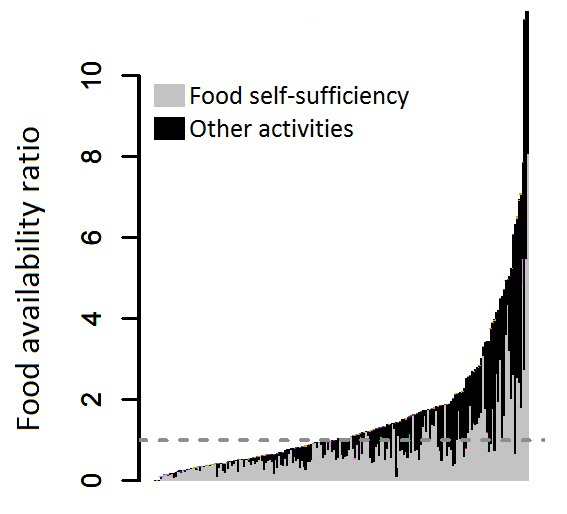
\includegraphics[width=0.5\textwidth]{figs_03/image1.png}
  \captionsetup{singlelinecheck = off, justification=justified} %left justify caption
  \caption{Food availability, food self-sufficiency and household energy needs: an example of unreliable values}
  \small
  %\raggedright
  \vspace*{-3mm}
  \caption*{Dashed line represents a case where 2,500 kilocalories are provided for each male adult equivalent \\
    (Source: \citealp{Rosenstock2017}; based on 200 households in northern Ghana)}
  \label{fig:03_1}
\end{figure}






\subsection{Consistency and reliability analyses}

In the consistency and reliability analyses we included variables that we would expect to be: a) highly consistent (age of the household head), b) relatively stationary in East Africa over the whole population over short time periods, including household size, productive assets (land owned and livestock holdings) and crop yields, and c) those that may be more variable (off-farm income, food availability and food self-sufficiency). Age of household head is expected to be highly consistent after accounting for the time elapsed between survey rounds and whether there was a change in household head. Household size was expected to be relatively stationary in East Africa given that death rates have been estimated to be less than 1\% per annum (\citealp{CIA2016a}) and the rate of urbanisation estimated to be less than 5.5\% per annum (\citealp{CIA2016}). Productive assets are also expected to be relatively stationary due to their livelihood and cultural value -- for both land (\citealp{Jayne2016}) and livestock (\citealp{Thornton2015}). Livestock holdings, however, are expected to be more temporally variable than land holdings due to their role in financing large expenditures, cultural utility (i.e. bride-wealth) and exposure to climatic and disease risks (ibid.). Similarly, crop yields are expected to be temporally stable (at a population level) in the absence of extreme weather events (\citealp{Gollin2006}). During the periods of observation, there were instances of extreme weather events, with a severe drought impacting northern Kenya and north-eastern Uganda (potentially impacting {\textless} 0.5\% of households in LSMS-ISA Uganda) and some evidence of increased extreme precipitation events in western Kenya, but to our knowledge this did not affect the sampled households (\citealp{Gebrechorkos2018}). Climatic conditions were consistent over the two survey rounds in Tanzania (\citealp{Fraval2018a}).

We explored the consistency of data collected in farm household surveys between two points in time, comparing respectively, IMPACTlite (2012) with RHOMIS (2015/16), and LSMS-ISA (2009/10 and 2011/12). Summary statistics of these changes between initial survey and revisit are provided in supplementary Information Table 3. In the absence of survey round specific biases, the correlations in these consistency results would provide a measure of reliability (\citealp{Alwin2006}). As this is not the case, we can only interpret the strength of correlation as a measure of consistency, rather than reliability. Spearman's correlation was used to assess association, as it is less sensitive to extreme non-credible values.

Reliability was more formally modelled using the core variables and derived indicators quantified from LSMS-ISA Uganda (2009/10, 2010/11, 2011/12), excluding some non-credible values. We used an approach described by \citet{Shrout1979} that calculates intraclass correlation (ICC). In this specification, we assume the following linear model:

\begin{equation}
\tag{3.1}
x_{ij}=\mu +b_{j}+w_{ij}
\end{equation}

Where x$_{\mathrm{ij}}$ is the value in the ith survey round (i = 1, 2, 3) of j household (j = 1, {\ldots}, n); $\mu$ is the population mean; b$_{\mathrm{j}}$ is the difference from $\mu$ to the jth household's mean across the survey rounds; w$_{\mathrm{ij}}$ is the residual, equal to the sum of the effects of survey round, survey round-household interaction, and error. The intraclass correlation is then estimated as follows:

\begin{equation}
\tag{3.2}
ICC=\frac{MSB-MSW}{MSB}
\end{equation}

Where MSB is the mean square between (sum of square total/obs) and MSW is mean square within, calculated as:

\begin{equation}
\tag{3.3}
\mathrm{MSW}=\frac{SS_{round}+SS_{resid}}{df_{round}+df_{resid}}
\end{equation}

For this analysis, some non-credible observations were excluded as they had a disproportionate influence on the linear models. Observations with off-farm income above US\$60,000 in one survey round were excluded (n = 1), as were maize yields above 15 tonnes per ha (n = 33), livestock holdings (TLU {\textgreater} 100, n = 3), land owned (ha {\textgreater} 100; n = 2) and food availability (FA {\textgreater} 1,500,000 kcal, n = 2). The reliability analysis was implemented using the psych package in R (\citealp{Revelle2017}). This analysis resulted in a reliability estimate ranging between 0 (`low reliability') and 1 (`high reliability') together with a 95\% confidence interval of this estimate. The three methodological steps and associated datasets, locations and years are summarised in Table \ref{tab:03_2}.



\begin{table}[H]
  \captionsetup{singlelinecheck = false, justification=justified} %left justify caption
  \caption{
  Summary of analysis, datasets and variables
  }
  \small
  \label{tab:03_2}
\begin{tabularx}{\textwidth}{@{}lllYYY@{}}
%  {
%p{\dimexpr 0.2\linewidth-2\tabcolsep}
%p{\dimexpr 0.21\linewidth-2\tabcolsep}
%p{\dimexpr 0.1\linewidth-2\tabcolsep}
%p{\dimexpr 0.16\linewidth-2\tabcolsep}
%p{\dimexpr 0.16\linewidth-2\tabcolsep}
%p{\dimexpr 0.16\linewidth-2\tabcolsep}}
\toprule
Survey tool & Country & Year & \multirow{2}{2cm}{Credibility (one round)} & Consistency (two rounds) & \multirow{2}{2.5cm}{Reliability (three rounds)} \\
\midrule
IMPACTlite & Kenya \& Tanzania & 2012 & x & a & \\
RHOMIS & Kenya \& Tanzania & 2015/16 & x & a & \\
LSMS-ISA & Uganda & 2009/10 & & b & c \\
LSMS-ISA & Uganda & 2010/11 & x & & c \\
LSMS-ISA & Uganda & 2011/12 & & b & c \\
LSMS-ISA & Tanzania & 2010/11 & x & & \\
LSMS-ISA & Ethiopia & 2010/11 & x & & \\
\bottomrule
\end{tabularx}
  \footnotesize
     \raggedright x = used in credibility assessment\\
     a, b, c = dataset, where two or three survey rounds are used in an analysis
\end{table}

%$\mathrm{ES}=\text{populationES}\times \sqrt \mathrm{r}$

The relationship between sample reliability, effect size and sample size was simulated using the `pwr' package in R (\citealp{Champely2018}), where reliability is mediated through the effect size ($ES = populationES \times \sqrt{r}$, assuming equal variace and sample sizes; \citealp{Phillips2016}). Using the pwr package, we simulated both a paired (panel type of data) and two-sample (Randomised Control Trial type of data) t-tests to quantify detectable differences for the core variables and derived indicators of which we have quantified reliability and uncertainty estimates. The simulated t-tests assumed a Type II error rate of 20\% (Power of 0.8) and a Type I error rate of 5\% (${\upalpha}$ of 0.05).

\section{Results}

\subsection{Credible bounds of core variables and derived indicators}

Yields and prices were highly variable in each of the three farm household survey tools. This variability across a wide range of crops could reflect agro-climatic or management differences, market volatility, as well as biases and errors introduced by the survey tool, enumerator or the respondent (\citealp{UnitedNationsDepartmentofEconomicandSocialAffairs2005}; \citealp{Mathiowetz2001}). This section provides a summary of non-credible values for yields (Table \ref{tab:03_3}), prices (Table \ref{tab:03_4}), food availability and food self-sufficiency (Table \ref{tab:03_5}).

Comparing our calculated maize yields with historical yield statistics compiled in the Global Yield Gap Atlas gives a reference point to assess yield estimates for each of the three survey tools. IMPACTlite had the highest proportion of households with crop yields less than 10\% of GYGA historical maize yields, followed by RHOMIS and then LSMS-ISA (Table \ref{tab:03_3}). On the other extreme, LSMS-ISA had the most substantial proportion of yields exceeding the simulated water-limited potential yield for the region -- occurring in 7\% of households. Four percent of households in LSMS-ISA 2010/11 Uganda exceeded potential maize yields and an additional 3\% were double this potential yield (Table \ref{tab:03_3}).



\begin{table}
  \captionsetup{singlelinecheck = false, justification=justified} %left justify caption
  \caption{Credibility of maize yield data: comparing enumerated yields with historical yields and water-limited potential yields, by survey tool* (proportion of households)
  }
  \small
  \label{tab:03_3}
\begin{tabularx}{\textwidth}{@{}lYYYY@{}}
%  {
%p{\dimexpr 0.22\linewidth-2\tabcolsep}
%p{\dimexpr 0.19\linewidth-2\tabcolsep}
%p{\dimexpr 0.27\linewidth-2\tabcolsep}
%p{\dimexpr 0.19\linewidth-2\tabcolsep}
%p{\dimexpr 0.13\linewidth-2\tabcolsep}}
\toprule
~ & Less than 10\% of historical yields & Greater than potential yield \& less than double & Double potential yield & Within bounds \\
\midrule
IMPACTlite 2012 & 0.43 & 0.00 & 0.01 & 0.56 \\
RHOMIS 2015/16 & 0.12 & 0.00 & 0.00 & 0.88 \\
LSMS-ISA 2010/11 & 0.03 & 0.04 & 0.03 & 0.90 \\
\bottomrule
\end{tabularx}
\footnotesize
\raggedright *Impact lite and RHOMIS include sites from Kenya and Tanzania, LSMS-ISA is limited to Uganda
\end{table}



Exceeding the simulated potential yield is possible, but unlikely -- even historical yields in optimal growing conditions were never more than 50\% of simulated potential yields (results not shown). It is more difficult, however, to assess the credibility of calculated yields at the lower end of the scale, which are far more prevalent. Comparing maize yields from the same sites from both IMPACTlite (2012) and RHOMIS (2015/16) data, 62\% of households that had yields less than one tonne per hectare had those low yields in both surveys. An additional tonne per hectare was reported by 27\% of households in the RHOMIS (2015/16) survey.

The farm-gate price per kilogram of maize was compared with the median price for each data collection instance as well as the market wholesale price (sourced from \citealp{FoodandAgricuturalOrganization2017}). The average market wholesale price of maize in Kampala, Uganda during the year of data collection was 20 US cents per kilogram, with a minimum of 11 cents. Approximately 15\% of LSMS-ISA (2011/12) Uganda crop prices exceeded the maximum wholesale price, and 1\% was below the lower threshold. There were also such potential credibility issues in the IMPACTlite and RHOMIS datasets, with maize prices exceeding maximum wholesale prices in 53\% and 14\% of cases respectively (Table \ref{tab:03_4}). Similar to yield, the lower range on price is more difficult to assess. There are product quality aspects, market timing and geographical differences also influencing price (particularly for LSMS-ISA in Uganda which aims to be nationally representative). These aspects could result in farm gate prices well below the regional average.



\begin{table}
  \captionsetup{singlelinecheck = false, justification=justified} %left justify caption
  \caption{
   Credibility of maize price data: comparing enumerated prices with average survey prices and wholesale market prices by survey tool* (proportion of households)
  }
  \small
  \label{tab:03_4}
\begin{tabularx}{\textwidth}{@{}lYYYY@{}}
  %{\textwidth}{
%p{\dimexpr 0.22\linewidth-2\tabcolsep}
%p{\dimexpr 0.19\linewidth-2\tabcolsep}
%p{\dimexpr 0.27\linewidth-2\tabcolsep}
%p{\dimexpr 0.19\linewidth-2\tabcolsep}
%p{\dimexpr 0.13\linewidth-2\tabcolsep}}
\toprule
~ & less than 10\% of average prices of survey & Greater than maximum wholesale price \& less than double & Double maximum wholesale price & Within bounds \\
\midrule
IMPACTlite 2012 & 0.03 & 0.50 & 0.03 & 0.43 \\
RHOMIS 2015/16 & 0.02 & 0.09 & 0.05 & 0.84 \\
LSMS-ISA 2010/11 & 0.01 & 0.11 & 0.04 & 0.84 \\
\bottomrule
\end{tabularx}
\footnotesize
\raggedright{*Impact lite and RHOMIS include sites from Kenya and Tanzania, LSMS-ISA is limited to Uganda}
\end{table}



Non-credible values in core variables will propagate through to composite indicators, such as food self-sufficiency and potential Food Availability (FA). Specifically, non-credible values in farm production, area planted, product marketing, off-farm income and household size can be compounded in these indicators. Table \ref{tab:03_5} shows the proportion of households that have non-credible food availability and self-sufficiency values (defined by being below half or more than double the energy demands of the household). Instances of non-credible FA values exist in all survey implementations, but more so in IMPACTlite. LSMS-ISA Uganda and LSMS-ISA Tanzania had the most non-credible food self-sufficiency values. LSMS-ISA Tanzania and Ethiopia are included in this table as an example of the variability in data quality generated with the same survey tool. LSMS-ISA Tanzania and Ethiopia appear to provide much lower quality food availability and food self-sufficiency estimates as compared to LSMS-ISA Uganda.





\begin{table}
  \captionsetup{singlelinecheck = false, justification=justified} %left justify caption
  \caption{
  Credibility of food availability (FA) and food self-sufficiency (FSS) by survey tool (proportion of households)
  }
  \small
  \label{tab:03_5}
\begin{tabularx}{\textwidth}{@{}lYYYY@{}} %{
%p{\dimexpr 0.29\linewidth-2\tabcolsep}
%p{\dimexpr 0.21\linewidth-2\tabcolsep}
%p{\dimexpr 0.27\linewidth-2\tabcolsep}
%p{\dimexpr 0.13\linewidth-2\tabcolsep}
%p{\dimexpr 0.09\linewidth-2\tabcolsep}}
\toprule
~ & Food availability less than 1250 kcal adult equivalent$^{-1}$ & FSS above OECD average \& Less than double & FSS double 2500 kcal adult equivalent$^{-1}$ & Within bounds \\
\midrule
IMPACTlite 2012 & 0.39 & 0.05 & 0.04 & 0.52 \\
RHOMIS 2015/16 & 0.15 & 0.06 & 0.04 & 0.75 \\
LSMS-ISA Uganda 2010/11 & 0.12 & 0.07 & 0.14 & 0.66 \\
LSMS-ISA Tanzania 2010/11 & 0.20 & 0.06 & 0.07 & 0.67 \\
LSMS-ISA Ethiopia 2010/11 & 0.40 & 0.02 & 0.07 & 0.51 \\
\bottomrule
\end{tabularx}
\footnotesize
\raggedright *Impact lite and RHOMIS include sites from Kenya and Tanzania
\end{table}


\newpage

\subsection{Consistency of core variable measurements and derived indicators over time}

After accounting for the time elapsed between the two surveys and excluding households where the household head had changed (LSMS-ISA, n = 168) or household head gender was different between rounds (IMPACTlite 2012-RHOMIS 2015/16, n = 67), 84\% of households in LSMS-ISA Uganda were within one year of the expected age. In contrast, only 47\% were within the expected range of one year in IMPACTlite-RHOMIS. The relationship between the successive surveys, as shown by Spearman's correlation coefficient in Figure \ref{fig:03_2}a, is strong in both LSMS-ISA (r = 0.99) and IMPACTlite-RHOMIS (r = 0.93). However, there were instances of substantial differences, with 1\% of households in LSMS-ISA, and 8\% of households in IMPACTlite-RHOMIS being 10 years greater or less at revisit than the expected age.

Household size was highly correlated between the 2009/10 and 2011/12 surveys in Uganda (r = 0.9) and moderately correlated in IMPACTlite-RHOMIS (r = 0.51; Figure \ref{fig:03_2}b). The majority of households in each dataset, however, remained within one adult equivalent of the initial visit. For instance, 62\% of households remained within one adult equivalent in LSMS-ISA and 55\% in IMPACTlite-RHOMIS (results not shown). There were isolated cases of extreme increases in each dataset, with the maximum increase in LSMS-ISA being 11 adult equivalents and 14 in IMPACTlite-RHOMIS (Figure \ref{fig:03_2}b).

\begin{figure}
  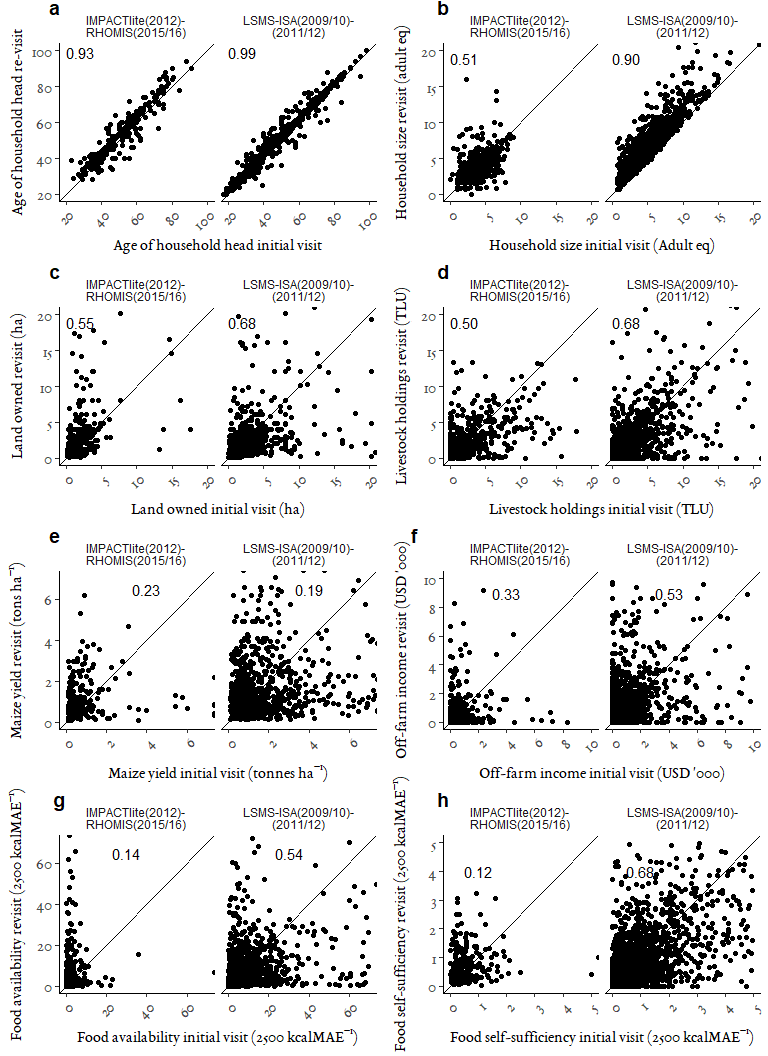
\includegraphics[width=1\textwidth]{figs_03/image2.png}
  \captionsetup{singlelinecheck = off, justification=justified} %left justify caption
  \caption{Consistency between IMPACTlite (2012)-RHOMIS (2015/16) in Kenya and Tanzania and LSMS-ISA (2009/10-2011/12) in Uganda*}
  \label{fig:03_2}
  %\small
  %\raggedright
  \vspace*{-3mm}
  \caption*{*Spearman's correlation coefficient (initial visit to revisit) indicated on each respective plot}
\end{figure}






Land owned in LSMS-ISA survey rounds had a higher correlation (r = 0.68) than IMPACTlite-RHOMIS (r = 0.55; Figure \ref{fig:03_2}c). Isolated cases of extreme changes in land owned were present in LSMS-ISA. Livestock holdings in LSMS-ISA Uganda had a Spearman's correlation coefficient of 0.68 between survey rounds. The level of association between rounds was lower in IMPACTlite-RHOMIS (r = 0.50; Figure \ref{fig:03_2}d). There was a similar level of correlation for maize yields in IMPACTlite-RHOMIS (r = 0.23) and LSMS-ISA (r = 0.19; Figure \ref{fig:03_2}e).

Off-farm income was moderately correlated between rounds in LSMS-ISA (r = 0.53) and less so in IMPACTlite-RHOMIS (r = 0.33; Figure \ref{fig:03_2}f). Changes in off-farm income of US\$5,000 or more occurred in 6\% of the households in Uganda and 2\% in IMPACTlite-RHOMIS. Households in LSMS-ISA, span a wide geographical range with varying proximity to urban locations which may explain such outliers.

Food availability at initial visit and revisit had a moderate association in LSMS-ISA (r = 0.54) and less so in IMPACTlite-RHOMIS (r = 0.14; Figure \ref{fig:03_2}g). There were instances of outliers in both survey comparisons; these few cases, however, could be realistic given large changes in on-farm and off-farm income. Food self-sufficiency followed a similar pattern to food availability, with LSMS-ISA having a having a greater level of correlation between survey rounds (r = 0.68) when compared to IMPACTlite-RHOMIS (r = 0.12; Figure \ref{fig:03_2}h).

Household diet diversity in the IMPACTlite-RHOMIS surveys also provides a notable case of inconsistency between survey rounds. For example, median increases in diet diversity range from three food categories in the lean peiod, and up to six food categories in the Tanzanian post-harvest period. As desirable as leaps in diet diversity are, it is unlikely to observe such a change over a short space of time in these communities (\citealp{IFAD2016}). Figure \ref{fig:03_3} shows the differences between the survey rounds in both periods for Tanzania as an example, where the same applies for IMPACTlite-RHOMIS in Kenya. The initial visit has instances where common food categories (e.g. fats and oils) are supposedly not consumed at all. The likely causes of these differences relate to survey design and duration. IMPACTlite enumerated a wide range of food items (not food groups) asked as an open question. Furthermore, these questions came at the end of a three-hour interview, potentially resulting in respondent fatigue. RHOMIS, on the other hand, asked about these food groups specifically and was completed within an hour.

\begin{figure}[H]
  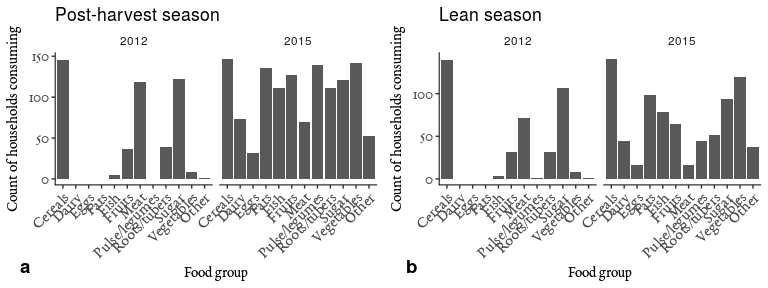
\includegraphics[width=0.8\textwidth]{figs_03/image3.png}
  \captionsetup{singlelinecheck = off, justification=justified}
  \caption{Diet diversity by category and period in IMPACTlite-RHOMIS Tanzania}
  \label{fig:03_3}
\end{figure}


\subsection{Reliability of variables in LSMS-ISA Uganda}

Modelling the reliability of variables explored in the consistency analysis provides further insight into the three waves in the LSMS-ISA Uganda case. The model outputs suggest a high degree of reliability for age, household size and livestock holdings (Figure \ref{fig:03_4}); land owned was less reliable than these other stationary variables and maize yield was one of the least reliable variables. It is more difficult to evaluate the reliability estimates of off-farm income, food availability and food self-sufficiency. The paucity of information about the temporal stability of these variables (despite efforts to assess the quality of variables such as income -- notably by \citealp{Neri2012}; \citealp{Fisher2010}; \citealp{Juster2007}; \citealp{Moore2000}) make it difficult to identify whether the reliability scores of these three variables are influenced by true population level temporal volatility, but it is clear that the reliability of these variables is low.

\begin{figure}[H]
  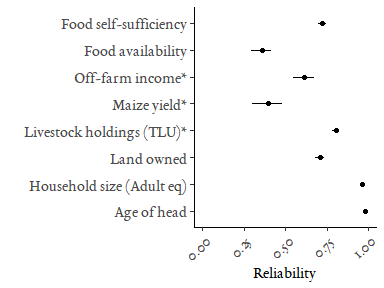
\includegraphics[width=0.5\textwidth]{figs_03/image4.png}
  \captionsetup{singlelinecheck = off, justification=justified}
    \caption{Reliability of initial visit variables in the living standards measurement survey, Uganda: output from intraclass correlations with 95\% Confidence Intervals}
  \label{fig:03_4}
  \small
  %\raggedright
  \vspace*{-3mm}
  \caption*{* Limited to households that were {\textgreater} 0 in each survey round. 27\% of households had off-farm income in all 3 rounds, 75\% cultivated maize, 60\% kept livestock}
\end{figure}




The reliability of these variables will ultimately affect inference as it reduces the power of tests (increasing Type II error) and inflates error estimates in multivariate analyses. Additionally, in instances of new studies using existing data for setting required sample sizes, consideration needs to be given to the reliability of available variables and how the proposed study will differ in terms of measurement error; a new study with a coarser measurement tool will require a larger sample than a previous study with more accurate measures. Figure \ref{fig:03_5} shows the relationship between sample reliability, effect size and sample size for paired and two-sample t-tests. For example, the sample size required to detect a relatively small effect size (0.2) in a paired test with a Type II error rate of 20\% and Type I error rate of 5\%, will be 220 with a reliability of 0.9 (as we see for household size) and 983 households for a reliability of 0.2 (as we see for off-farm income and crop yield). These sample sizes will be higher when design effects are incorporated and when two-sample tests are needed.

\begin{figure}[H]
  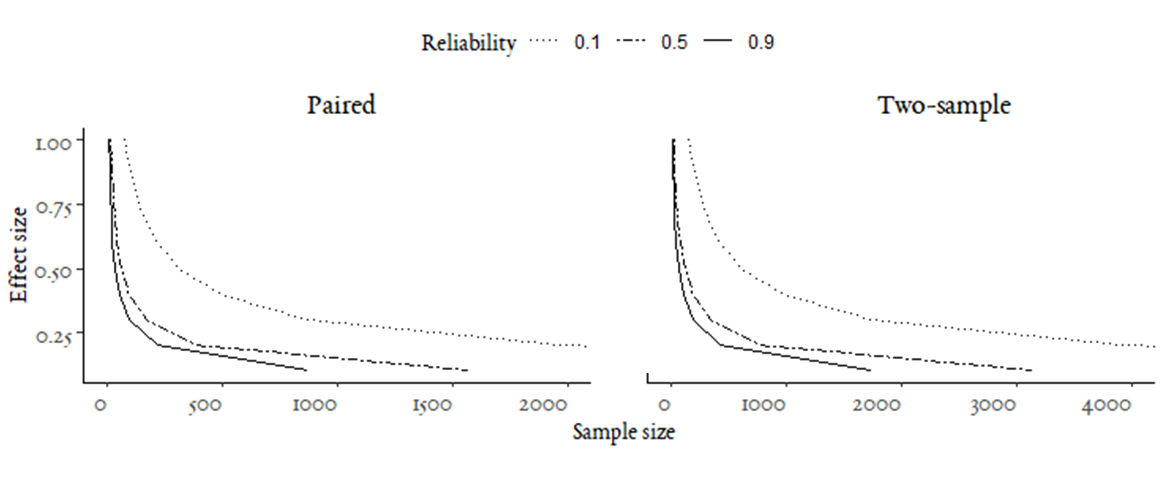
\includegraphics[width=0.8\textwidth]{figs_03/image5.png}
  \captionsetup{singlelinecheck = off, justification=justified}
  \caption{Sample size and effect size given different levels of reliability for t-test (power = 0.8; ${\upalpha}$ = 0.05)}
  \label{fig:03_5}
\end{figure}


\section{Discussion}

\subsection{Credibility of crop yield and market price}

Using data from three cross-sectional farm household survey approaches, we assessed the credibility and reliability of core variables and derived indicators. This study has identified quality limitations in each survey tool -- with LSMS-ISA and RHOMIS staying within credible bounds more frequently than IMPACTlite (Tables \ref{tab:03_3} and \ref{tab:03_4}). The higher performance of these two survey tools may be due to their innovative data collection strategies -- particularly in the case of enumerating cropping activity. In the case of LSMS-ISA, enumerators visit households each cropping season -- with the intention of minimising recall error. In the case of RHOMIS, households can quantify harvest volumes in a unit of their choice (such as standard sized sacks) rather than force kilogram estimates -- minimising error due to respondent estimation. These innovations are positive, however they are not sufficient to eliminate non-credible values.

\subsection{Consistency of variables between two survey rounds}

The inconsistencies identified in this study -- including age of household head, household size (Figure \ref{fig:03_2}) and diet diversity (Figure \ref{fig:03_3}) -- reinforce the notion that researchers need to consider their data collection strategy for each variable rather than assuming that some are `easy' to enumerate. In the instance of diet diversity, the differences between survey rounds may be explained by an unfortunate combination of question design and survey length. The data collection strategy of IMPACTlite, in this instance, was to ask an open question -- ``what food items did you consume?'' -- and allow the enumeration of a detailed list of food items. These questions on diet diversity, however, came at the end of more than two hours of questions and so the quality of data may have suffered from the farmer (and enumerator) being fatigued (as systematically explored by \citealp{Kilic2013}).

\subsection{Implications of the lower reliability over three survey rounds}

The lack of reliability of land owned and crop yields variables has implications in the monitoring of food security status, poverty status and land productivity of households. These variables are also used to answer essential questions of cause and effect and can have a substantial bearing on policy decisions. For instance, the question of whether smaller farms are more productive than larger farms in developing countries has implications for reducing yield gaps and has been an active area of debate. Recently, the robustness of the data underpinning the analysis of this relationship was tested using LSMS-ISA data. In order to test the robustness of underpinning data, farmer reported values were compared against Global Positioning System (GPS) based land area estimates (\citealp{Kilic2013}; \citealp{Carletto2011}). These studies found that despite measurement error in farmer reported values, the inverse productivity relationship was still detected.

The implications of non-credible values and lower reliability are more pronounced in composite indicators such as food self-sufficiency and food availability -- where the uncertainty propagates from multiple variables. This leads to i) substantial portions of the survey results to be beyond credible bounds (Table \ref{tab:03_5}); ii) the need for larger sample sizes so that change and differences between groups can be detected (Figure \ref{fig:03_5}), and; iii) limitations in identifying relationships in multivariate analysis, such as food availability and agricultural land use strategies (among households and over time).

\subsection{Data quality in perspective -- sample sizes, continuous improvement and transparency}

Despite this seemingly bleak picture of data quality of variables derived from farm household surveys, there is still cause for optimism. First, the sample sizes needed to detect substantial changes (which are often the changes of interest in agricultural development research) in the variables assessed in this study are in the hundreds, and not in the thousands such as for a Randomised Control Trial (see Figure \ref{fig:03_5}). With tight controls on quality and a less variable population to represent, this sample size can be even smaller. The second cause for optimism is that ongoing developments in data collection strategies and tools are likely to improve data quality and reduce measurement error. There have been many areas of progress in the last 10 years that have improved quality including: harmonised survey tools, in-country capacity building, mixed modes of data collection (e.g. GPS data, phone, SMS; \citealp{Carletto2016}; \citealp{Deininger2011}; \citealp{Leeuw2005}), quality control protocols (e.g. rapid data quality checks and variable triangulation; \citealp{Fisher2010}) and non-paper based collection (\citealp{Rosenstock2017}).

An example of a new, more systematised household survey is RHOMIS (\citealp{Hammond2017225}). The evaluations in this study show that such targeted data collection does result in highly credible quantification of indicators like food self-sufficiency and food availability (e.g. Table \ref{tab:03_5}). RHOMIS furthermore assesses food security by quantifying clusters of indicators rather than a single indicator (Household Diet Diversity score, the USAID Hunger and Food Insecurity Access scale, Food Availability and the number of hunger months as indicators), thereby allowing for a more integral picture of food security. These benefits do have some limitations when used to follow up on households that have been surveyed with different tools, where Figure \ref{fig:03_3} shows inconsistencies and thus a potential to increase Type II error - not having the power to identify significant differences between communities and over time.

The third cause for being optimistic about the use of household-based rural statistics is that the survey tools analysed in this study were transparent about sampling and data collection procedures. This practice informs data users of what the sample is representative of, and the nature of the questions asked. Such transparency guides the secondary utilisation of these data and can reduce misuse and misinterpretation.

\subsection{Improving the quality of farm household survey data}

Several steps can be taken to improve the data quality of farm household surveys further. First, researchers can compare a subset of collected data to the `truth', where there is a possibility to collect detailed data from a smaller subset of households (referred to as `two method measurement designs', \citealp{Little2013}) which is widely accepted to be of far greater reliability and accuracy (as demonstrated by \citealp{Giller2011}). For instance, plot sizes of a sub-sample might be measured using Global Positioning System (GPS) receivers or through remote sensing, providing a more consistent level of accuracy across households. Secondly, researchers can analyse data for reliability (as done in this study) and potential instances of data fraud (as discussed in \citealp{Finn2017}) which would highlight issues that could improve overall quality.

Rural sub-Saharan Africa is entering a stage of transformation where the opportunities and challenges for rural communities are becoming more pronounced, and at the same time, the means of gaining insight into these communities is broadening. In this setting, the fundamentals of generating fit-for-purpose and representative observations remain a vital basis for informed decision making. For decision makers to make the most of such inherently coarse data, it is essential to have the foundation of robust sampling, quality-centric survey design (questions and length), transparency of experimental design and effective training. The quality and usability of such data can be further enhanced by improving coordination between agencies, incorporating mixed modes of data collection and continuing systematic validation programs.

\section{Acknowledgements}

We are grateful to the research teams who were involved in designing and implementing the three surveys assessed in this study. Without their rigor, openness and thorough documentation this study would not have been possible. We also thank the two anonymous reviewers and special edition editor Jens Andersson, whose comments and suggestions greatly improved the quality of this article. This study was made possible by the CGIAR Research Program on Livestock and its donors and by support of the American People provided to the Feed the Future Innovation Lab for Sustainable Intensification through the United States Agency for International Development (USAID). The views expressed in this paper cannot be taken to reflect the official opinions of these organisations.
